%---------------------------------
%---------------------------------
%---------------------------------
\section{RVV memory instructions\label{chap:bg:sec:rvvmemory}}
\emph{Summarizes \cite[Sections 7-9]{RISCVVectorExtension2021}}

RVV defines three broad categories of memory access instructions, which can be further split into five archetypes with different semantics.
This section summarizes each archetype, their semantics, their assembly mnemonics, and demonstrates how they map memory accesses to vector elements.

% \begin{table}[]
%     \centering
%     \begin{tabular}{cc|c|}
%     \toprule
%         Archetype & Direction &  Category \\
%         \midrule
%         Unit/Strided & Load/Store & Unit/Strided \\
%         Fault-only-First & Load & Unit \\
%         Whole-Register & Load/Store & Unit \\
%         Bytemask & Load/Store & Unit \\
%         Indexed & Load/Store & Indexed
%         \bottomrule
%     \end{tabular}
%     \caption{Table of categories/archetypes??}
%     \label{tab:my_label}
% \end{table}

% RVV defines five broad categories of memory access instructions.
For the most part, memory access instructions handle their operands as described in \cref{chap:bg:sec:rvv:vector_model}.
\code{EEW} and \code{EMUL} are usually derived from the instruction encoding, rather than reading the \code{vtype} CSR.
In a few cases the Effective Vector Length \code{EVL} is different from the \code{vl} CSR, so for simplicity all instructions are described in terms of \code{EVL}.

\subsection{Segmented accesses}
Three of the five archetypes (unit/strided, fault-only-first, and indexed) support \emph{segmented} access.
This is used for unpacking contiguous structures of $1 \le \code{nf} \le 8$ \emph{fields} and placing each field in a separate vector.
In these instructions, the values of \code{vl}, \code{vstart}, and the mask register are interpreted in terms of segments.
% Additionally, if an element within a segment causes a synchronous exception/trap, it

\cref{fig:RVV_mem_unit} demonstrates a common example: the extraction of separate R, G, and B components from a color.
Without segmentation, i.e. $n = 1$, each consecutive memory address maps to a consecutive element in a single vector register group.
With segmentation, elements are grouped into segments of $n > 1$ fields, where each field is mapped to a different vector register group.
This principle extends to \code{LMUL > 1} (\cref{fig:RVV_mem_lmul_3seg}).

% \todomark{vl, vstart, masks are all in terms of segments in segmented accesses.}
% \todomark{if a trap occurs, it is implementation defined if a subset of the faulting segment's accesses are performed before the trap is taken}
% \todomark{nf has range 1..8}

\figinput[width=0.48\textwidth,pos=h]{1_20Background/figures/fig_RVV_mem_unit}
% \figinput[width=0.55\textwidth,pos=h]{1_20Background/figures/fig_RVV_mem_lmul_3seg}


\pagebreak
%%%%%%%%%%%%%%%%%%%%%%%%%%%%%%%%%%%%%%%%%%
\subsection{Unit and Strided accesses}\label{chap:bg:sec:rvv:unitstrideaccess}

\begin{figure}[h]
    \centering
    \begin{subfigure}{\textwidth}
        \centering
        \large (Unit) \code{vlseg\param{<nf>}e\param{<eew>}.v vd, (rs1), vm} \\
(Strided) \code{vlsseg\param{<nf>}e\param{<eew>}.v vd, (rs1), rs2, vm}
        \caption{Instruction}
    \end{subfigure}
    \vspace{1em}
    
    \begin{subtable}[b]{0.5\textwidth}
    \begin{tabular}{ll}
    \toprule
    Masked? & \code{vm == 0} \\
        \code{stride} & (Unit) \code{\param{<eew>} * \param{<nf>}} \\
                    & (Strided) From \code{rs2} \\
        \code{EEW} & \paramt{<eew>} \\
        \code{EVL} & \code{vl} \\
        \code{EMUL} & \code{VLEN * \param{<eew>} / EVL} \\
        \code{NFIELDS} & \paramt{<nf>} \\
        \bottomrule
    \end{tabular}
    \caption{How fields are interpreted}
    \label{tab:RVV_mem_strided}
    \end{subtable}\hfill
    \begin{subfigure}[b]{0.5\textwidth}
        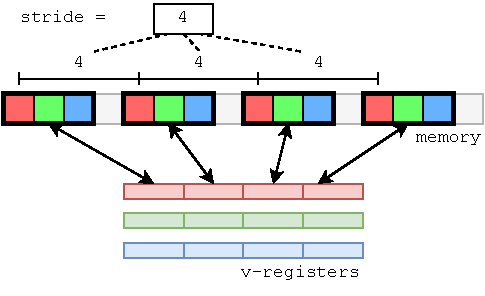
\includegraphics[width=\textwidth]{Figures/RVV_mem_strided_3seg.pdf}
        \caption{Example of a segmented strided access\\\code{EEW=8-bits}, \code{nf=3}, \code{stride=4},\code{EVL=4}}
        \label{fig:RVV_mem_strided_3seg}
    \end{subfigure}
    \caption{Segmented Unit/Strided Access Information}
\end{figure}

\noindent
Moves active elements of \paramt{nf} vector register groups to/from contiguous segments of memory,
where each segment is separated by \code{stride} bytes.

\begin{itemize}
    \item The start of each segment is separated by \code{stride} bytes.
    \begin{itemize}
        \item The Unit version (short for Unit-stride) tightly packs segments, equivalent to selecting \code{stride = \param{nf} * \param{eew} / 8}.
        \item \code{stride} may be negative or zero.
        \item If \code{rs2} is register \code{x0}, implementations may perform fewer than \code{EVL} memory accesses. Otherwise, they must appear to perform all memory accesses, even if the value of \code{rs2} is zero.
    \end{itemize}
    % These two are described by the diagram
    % \item Each segment is \code{\param{nf} * \param{eew}} bits long, i.e. \paramt{nf} elements long.
    % \item Each element in the $i$-th segment maps to the $i$-th element of a vector register group.
    \item This instruction doesn't do anything if the \code{vstart >= EVL}.
\end{itemize}


% ORDERING
\subsubsection*{Ordering}
There are no ordering guarantees, other than those required by precise vector traps (if used).

% EXCEPTION HANDLING
\subsubsection*{Exception Handling}
If any element within segment $i$ triggers a synchronous exception, \code{vstart} is set to $i$ and a precise or imprecise trap is triggered.
Load instructions may overwrite active segments past the segment index at which the trap is reported, but not past \code{EVL}.\cite[Section 7.7]{RISCVVectorExtension2021}
Upon entering a trap, it is implementation-defined how much of the faulting segment's accesses are performed.

\subsection{Unit fault-only-first loads}\label{chap:bg:sec:rvv:fof}

\begin{table}[h]
    \centering
\begin{tabular}{ll}
\multicolumn{2}{c}{\large \code{vlseg\param{<nf>}e\param{<eew>}ff.v vd, (rs1), vm}} \\
    \toprule
    Masked? & \code{vm == 0} \\
        \code{EEW} & \paramt{<eew>} \\
        \code{EVL} & \code{vl} \\
        \code{EMUL} &  \code{VLEN * \param{<eew>} / EVL} \\
        \code{NFIELDS} & \paramt{<nf>} \\
    \bottomrule
\end{tabular}
    \caption{Unit Fault-only-First Information}
    \label{tab:RVV_mem_fof}
\end{table}

This is equivalent to a unit load in all respects but exception handling.
If any access in segment 0 raises an exception\footnote{Segment 0 may be masked out, in which case this is impossible.}, \code{vl} is not modified and the trap is taken as usual.
If any access in any active segment $> 0$ raises an exception, the trap is not taken, \code{vl} is reduced to the index of the offending segment, and the instruction finishes.
If an asynchronous interrupt is encountered at any point, the trap is taken and \code{vstart} is set as usual.

Similar to plain loads, if an exception is encountered the instruction is allowed to update segments past the offender (but not past the original \code{vl}).
If any synchronous exception or asynchronous interrupt occurs, regardless of the segment index, it is implementation-defined how much of the faulting segment's accesses are performed.

\pagebreak
%%%%%%%%%%%%%%%%%%%%%%%%%%%%%%%%%%%%%%%%%%
\subsection{Indexed accesses}
\begin{figure}[h]
    \centering
    \begin{subfigure}{\textwidth}
        \centering
        \large \code{vl\param{<u|o>}xseg\param{<nf>}e\param{<eew>}.v vd, (rs1), vs2, vm}
        \caption{Instruction}
    \end{subfigure}
    \vspace{1em}
    
    \begin{subtable}[b]{0.5\textwidth}
    \begin{tabular}{ll}
    \toprule
        Masked? & \code{vm == 0} \\
    \midrule
        Element \code{EEW} & \code{vtype.SEW} \\
        Element \code{EMUL} & \code{vtype.LMUL} \\
        \midrule
        Ordered? & \paramt{<u|o>} \\
        Index Vector & \code{vs2} \\
        Index \code{EEW} & \paramt{<eew>} \\
        Index \code{EMUL} & \code{VLEN * \param{<eew>} / EVL} \\
        \midrule
        \code{NFIELDS} & \paramt{<nf>} \\
        \code{EVL} & \code{vl} \\
        \bottomrule
    \end{tabular}
    \caption{How fields are interpreted}
    \label{tab:RVV_mem_index}
    \end{subtable}\hfill
    \begin{subfigure}[b]{0.5\textwidth}
        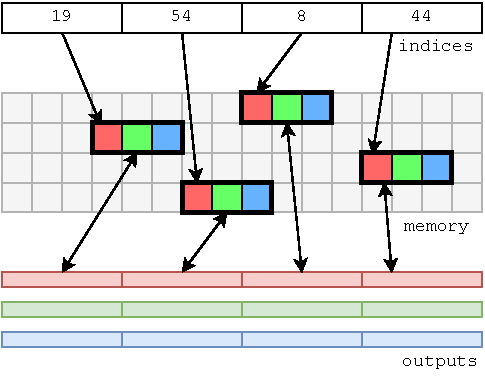
\includegraphics[width=\textwidth]{Figures/RVV_mem_index_3seg.pdf}
        \caption{Example of a segmented indexed access\\\code{EEW=8-bits}, \code{nf=3}}
        \label{fig:RVV_mem_index_3seg}
    \end{subfigure}
    \caption{Segmented Indexed Access Information}
\end{figure}

Moves elements of \paramt{nf} vector register groups to/from contiguous segments of memory,
where each segment is offset by an index (in bytes) taken from another vector.

\begin{itemize}
\item The start of each segment is defined by \code{base address + index\_vector[i]}.
\item This instruction doesn't do anything if \code{vstart >= EVL}.
\end{itemize}

% ORDERING
\subsubsection*{Ordering}
Accesses within each segment are not ordered relative to each other.
If the ordered variant of this instruction is used, then the segments must be accessed in order (i.e. 19, 54, 8, 44 for \cref{fig:RVV_mem_index_3seg}).
Otherwise, segment ordering is not guaranteed.


% EXCEPTION HANDLING
\subsubsection*{Exception Handling}
If any element within segment $i$ triggers a synchronous exception, \code{vstart} is set to $i$ and a precise or imprecise trap is triggered.
Load instructions may overwrite active segments past the segment index at which the trap is reported, but not past \code{EVL}\cite[Section 7.7]{RISCVVectorExtension2021}.
Upon entering a trap, it is implementation-defined how much of the faulting segment's accesses are performed.

\pagebreak
\subsection{Unit whole-register accesses}

\begin{table}[h]
    \centering
\begin{tabular}{ll}
    \multicolumn{2}{c}{\large \code{vl\param{<nreg>}re\param{<eew>}.v vd, (rs1)}} \\
\toprule
        Masked? & False \\
        Number of Registers & \paramt{<nreg>} \\
        \code{EEW} & \paramt{<eew>} \\
        \code{EVL} & \code{NFIELDS * VLEN / EEW} \\
        \code{EMUL} & 1 \\
    \bottomrule
\end{tabular}
    \caption{Unit Whole Register Information}
    \label{tab:RVV_mem_wholereg}
\end{table}

Moves the contents of \paramt{nreg} vector registers to/from a contiguous range in memory.
Equivalent to a unit-stride access where \code{EVL} equals the total number of elements in \paramt{nreg} registers.
\begin{itemize}
    \item \code{nreg} must be a power of two.
    \item Doesn't support segmented access.
    \item This instruction doesn't do anything if \code{vstart >= EVL}.
\end{itemize}

Ordering and exception handling are identical to unit-stride accesses (\cref{chap:bg:sec:rvv:unitstrideaccess}).

\subsection{Unit bytemask accesses}
\begin{table}[h]
    \centering
\begin{tabular}{ll}
\multicolumn{2}{c}{\large \code{vlm.v vd, (rs1)}} \\
    \toprule
        Masked? & False \\
        \code{EEW} & 8-bits \\
        \code{EVL} & \code{ceil(vl/8)} \\
        \code{EMUL} & 1 \\
    \bottomrule
\end{tabular}
    \caption{Unit Bytemask Information}
    \label{tab:RVV_mem_bytemask}
    % \end{subtable}\hfill
\end{table}

Moves the contents of a mask register to/from a contiguous range of memory.
This instruction transfers at least \code{vl} bits,
one bit for each element that could be used in subsequent vector instructions.
This will always fit in a single vector register (see \cref{chap:bg:sec:rvv:masking}), hence \code{EMUL = 1} in all cases.
\begin{itemize}
    \item This instruction always operates as if the tail-agnostic setting of \code{vtype} is true.
    \item This instruction doesn't support segmented access.
    \item This instruction doesn't do anything if \code{vstart >= EVL}.
\end{itemize}
Ordering and exception handling are identical to unit-stride accesses (\cref{chap:bg:sec:rvv:unitstrideaccess}).